\documentclass{article}

\PassOptionsToPackage{numbers, compress, sort}{natbib}
\usepackage[final]{neurips_2025}

% This is a course project report, not a NeurIPS paper: replace the conference footer.
\makeatletter
\renewcommand{\@noticestring}{B.Tech Computer Vision course project, IIT Jodhpur, November 2026.}
\makeatother

\usepackage[utf8]{inputenc}
\usepackage[T1]{fontenc}
\usepackage{hyperref}
\usepackage{url}
\usepackage{booktabs}
\usepackage{amsfonts}
\usepackage{amsmath,amssymb}
\usepackage{nicefrac}
\usepackage{microtype}
\usepackage{xcolor}
\usepackage{graphicx}
\usepackage{array}
\usepackage{tikz}
\usetikzlibrary{positioning,arrows.meta,fit,backgrounds,calc}

\hypersetup{colorlinks=true, linkcolor=black, citecolor=black, urlcolor=black}

\definecolor{ink}{HTML}{2B2B2B}
\definecolor{repoblue}{HTML}{0B57D0}
\definecolor{edge}{HTML}{6B6B6B}
\definecolor{ours}{HTML}{EEF2F6}
\definecolor{ourline}{HTML}{4A5E78}
\definecolor{pre}{HTML}{F6EAD7}
\definecolor{preline}{HTML}{B07A2A}

\newcommand{\unet}{U$^2$-Net}
\newcommand{\tl}[1]{\makebox[0.1404\textwidth]{\scriptsize #1}\hspace{0.0028\textwidth}}
\newcommand{\tlast}[1]{\makebox[0.1404\textwidth]{\scriptsize #1}}

\title{Trycraz: Diffusion-Based Virtual Try-On with\\Context-Aware Clothing Recommendation}

\author{%
  Darshan Prajapati \\
  Chemical Engineering \\
  Indian Institute of Technology Jodhpur \\
  Roll No: B23CH1032 \\
  \And
  Sunny Kumar \\
  Mechanical Engineering \\
  Indian Institute of Technology Jodhpur \\
  Roll No: B23ME1073 \\
}

\begin{document}

\maketitle

\vspace{-1.2em}
\begin{center}
\setlength{\fboxsep}{6pt}%
\fcolorbox{repoblue}{white}{\normalsize\textbf{\textcolor{repoblue}{GitHub repository:\ \href{https://github.com/CrazAzartto/trycraz-virtual-tryon}{https://github.com/CrazAzartto/trycraz-virtual-tryon}}}}
\end{center}
\vspace{0.4em}

\begin{abstract}
Virtual try-on shows how a garment would look on a person, but it does not say whether that garment
suits the place the person is going to. We built Trycraz, a working system that answers both questions.
A user uploads a photo and a garment, and the pretrained CatVTON diffusion model renders the person
wearing it. A context-aware recommender ranks a 52-garment catalogue for a given occasion, setting and
weather, explains every score in plain words, and sends any pick straight to the try-on. We did not
train the generator. Our work is the system around it: input validation, a pose-based quality gate
built on MediaPipe, garment background removal with \unet, a job-based GPU server that runs on a free
Colab or Kaggle T4, a hybrid recommender that combines hand-written dress-code knowledge with CLIP
zero-shot scores, and a Streamlit application. On a T4 a try-on takes 61.5--62.4\,s for 30 denoising
steps with a peak of 4.89\,GB of GPU memory. Our first real runs had two clear failures; diagnosing
them one hypothesis at a time showed that a photo cut off at the hips, not the garment, was the cause.
After adding a framing rule and background removal, all six validation try-ons succeeded. On twelve
labelled scenarios the hybrid recommender reaches a mean P@5 of 0.833 and nDCG@5 of 0.830, higher
than either attribute rules (0.767/0.751) or CLIP alone (0.667/0.691).
\end{abstract}

\section{Introduction}
\label{sec:intro}

When people shop for clothes online, two questions come up again and again: \emph{how will this look
on me}, and \emph{is it right for where I am going}. Image-based virtual try-on addresses the first
one. Given a photo of a person and a photo of a garment, a try-on model produces a new photo of that
person wearing the garment, while keeping their face, body shape, pose and background. Recent
diffusion models have made these results realistic enough to be useful. They still say nothing about
the second question, so a user can get a convincing picture of themselves in a hoodie without being
told that a hoodie is a poor choice for a job interview.

Trycraz combines the two. The user chooses whether they are shopping for menswear or womenswear, then
describes the occasion (for example interview, college or wedding), the setting (indoor or outdoor) and
the weather. The system ranks a catalogue, explains each score, and lets the user try any
recommendation on with one click. The try-on result is shown with a drag-to-compare slider and a
verdict on how well the garment suits the chosen occasion.

The image synthesis is done by CatVTON~\cite{catvton}, a pretrained model that we use as published.
We chose it because it is the lightest of the current diffusion try-on models, handles tops, bottoms
and dresses, and builds its own clothing mask. Everything else in this report is our own work. The
main contributions are:
\begin{itemize}
\item an end-to-end system that runs a 899\,M-parameter diffusion model on a free cloud T4 and serves
it to a laptop app over an authenticated tunnel, with progress reporting and clear error messages;
\item a pre-generation quality gate that uses pose landmarks to catch photos that are likely to fail,
including a rule we derived from a real failure: photos cut off at the hips;
\item a hybrid, explainable recommender whose six factor scores produce both the ranking and the
explanation, so the two can never disagree;
\item an honest evaluation: timing and memory on real hardware, a hypothesis-by-hypothesis failure
analysis, ranking metrics with an ablation, and 166 automated tests.
\end{itemize}


The rest of this report is organised as follows. Section~\ref{sec:lit} reviews earlier work on
virtual try-on, the models we build on, and outfit recommendation. Section~\ref{sec:problem} states
the problem and the constraints we worked under. Section~\ref{sec:method} describes the proposed
method: the system, the try-on model, our own pipeline around it, the recommender and the
optimisations we made. Section~\ref{sec:exp} reports the experiments and results, including a failure
analysis and a discussion of limitations, and Section~\ref{sec:concl} concludes.

\section{Literature Review}
\label{sec:lit}

\paragraph{Warping-based virtual try-on.}
Early try-on methods split the problem in two: first warp the garment to the body, then blend it in.
VITON-HD~\cite{vitonhd} raised the resolution to 1024$\times$768 with a GAN and a normalisation layer
that handles misalignment between the warped garment and the body. Warping methods still break when
the pose is unusual or the garment is loose, because one geometric transform cannot describe how cloth
folds.

\paragraph{Diffusion-based virtual try-on.}
Diffusion models changed this. Latent diffusion~\cite{ldm} runs the denoising process in the
compressed latent space of an autoencoder, which makes 1024-pixel images affordable. IDM-VTON~\cite{idmvton}
builds on two SDXL-sized networks, one for the person and one for the garment, and gives very good
results, but it needs far more memory than a free GPU offers. CatVTON~\cite{catvton} takes the
opposite route. It removes the second network and the text encoder altogether, and simply places the
person and the garment side by side in one image, as described in Section~\ref{sec:catvton}.
Because the person and garment share one self-attention space, CatVTON learns garment placement
implicitly. That keeps it small enough for the free hardware available to us, which is the
main reason we chose it.

\paragraph{Human parsing, pose and segmentation.}
Every try-on method needs to know which pixels belong to the clothing that will be replaced. DensePose~\cite{densepose}
maps each body pixel to a body-part surface, and Self-Correction for Human Parsing (SCHP)~\cite{schp}
labels pixels as hair, face, upper clothes, trousers and so on. CatVTON combines the two to build its
clothing mask. Lighter models are useful outside the generator too: BlazePose~\cite{blazepose} finds 33
body landmarks in real time on a CPU, and \unet~\cite{u2net}, a nested U-structure for salient object
detection, separates a foreground object from its background without class labels. We use these two
to check and clean the inputs before any GPU time is spent.

\paragraph{Outfit recommendation and zero-shot vision--language models.}
Most published outfit recommenders learn compatibility between garments, or between a garment and a
setting, from large labelled fashion datasets. We had no such data for occasions and weather, so we
wrote the dress-code knowledge by hand. To let the system look at the garment photo itself, we added
CLIP~\cite{clip}, a vision--language model trained on image--text pairs, which can score an image
against a text description such as ``formal clothes for a job interview'' without any training on our
data. Combining rules with zero-shot scores keeps every decision explainable.

\paragraph{Gap.} Try-on systems show how a garment looks but not whether it suits the situation, and
recommenders suggest garments without showing them on the user. The open-source try-on demos we tried,
including CatVTON's own, stop at the image. Our project connects the two: an explainable,
context-aware recommender whose suggestions can be tried on in one step.

\section{Problem Statement}
\label{sec:problem}

We address two coupled tasks.

\paragraph{Task 1: virtual try-on.} Given a photo $I_p$ of a person, a photo $I_g$ of a garment and the
garment's category $\tau\in\{\text{upper},\text{lower},\text{overall}\}$, produce an image $\hat I$ in which
the same person wears the garment. Outside the region the garment covers, $\hat I$ should match $I_p$:
the face, hair, hands, pose, body shape and background must not change. Inside it, the garment's colour,
pattern, text and shape should be carried over faithfully and draped to the person's pose.

\paragraph{Task 2: context-aware recommendation.} Given a catalogue $\mathcal G=\{g_1,\dots,g_N\}$ of
garments and a context $c=(a, o, s, w, p)$, consisting of the wear line $a$ (menswear or womenswear), the
occasion $o$ (one of 9), the setting $s$ (indoor or outdoor), the weather $w$ (one of 4) and optional
colour, style and formality preferences $p$, return:
\begin{itemize}
\item a ranking of the suitable garments by a score $S(g,c)\in[0,1]$;
\item for every ranked garment, a short explanation that agrees with its score;
\item the garments that are clearly unsuitable (for example shorts for an interview), listed
separately with a reason.
\end{itemize}
The user must be able to send any recommended garment straight to Task~1, and to ask whether a garment of
their own suits the context.

\paragraph{Constraints.} The problem is shaped as much by our constraints as by the tasks:
\begin{enumerate}
\item \emph{No local GPU capable of diffusion.} Our laptop has an RTX~3050 with 4\,GB of VRAM and
7.6\,GB of RAM. The only GPUs available to us are free, time-limited Colab and Kaggle T4 sessions, which
can disconnect.
\item \emph{No training data for suitability.} There is no public dataset that labels garments by
occasion and weather in a way we could train on, and we have no budget to train or fine-tune a try-on
model.
\item \emph{Uncontrolled inputs.} Users take photos at home: partial framing, cluttered
backgrounds, poor light. The try-on models we found were trained on studio photos.
\item \emph{Trust.} A recommendation is only useful if the user can see why it was made, so every
score must be explainable, and the explanation must not contradict the score.
\end{enumerate}

\paragraph{Success criteria.} For Task~1: realistic results on front-facing photos, judged visually,
with a response time of about one to two minutes, and memory that fits a T4. For Task~2: ranking
quality on labelled scenarios, measured by Precision@5 and nDCG@5, and rankings that change with the
context. For the system as a whole: clear messages instead of crashes when inputs or the server go
wrong, verified by automated tests.

\section{Proposed Method}
\label{sec:method}

\subsection{System Overview}
\label{sec:overview}

Fig.~\ref{fig:arch} shows the system. It is split across two machines because the diffusion model
does not fit on our laptop (an RTX~3050 with 4\,GB of VRAM and 7.6\,GB of system RAM). The laptop runs
the Streamlit app, the input checks, background removal, CLIP and the recommender, all on the CPU. The
try-on model runs on a free Google Colab or Kaggle notebook with an NVIDIA T4 (16\,GB). The notebook
starts a small FastAPI server and exposes it through a Cloudflare quick tunnel, so the laptop reaches it
over HTTPS with an API key.

\begin{figure}[t]
\centering
\resizebox{\linewidth}{!}{%
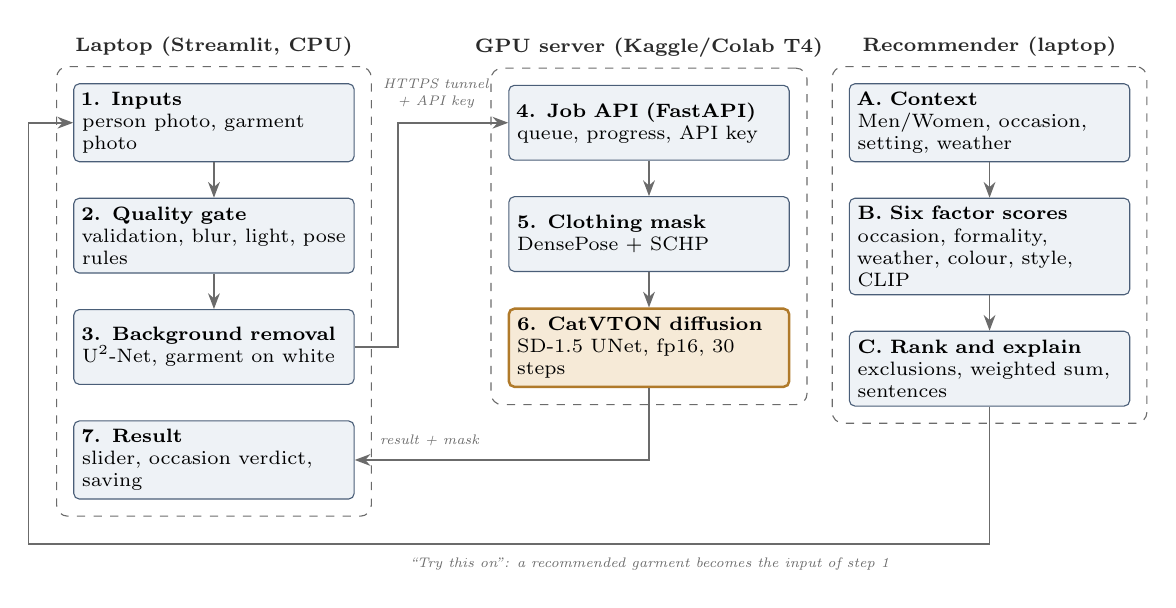
\begin{tikzpicture}[
  font=\scriptsize, >={Stealth[length=2mm]},
  box/.style={draw=ourline, fill=ours, rounded corners=2pt, align=left, text width=3.35cm, minimum height=0.95cm, inner sep=3pt},
  pbox/.style={draw=preline, fill=pre, line width=0.9pt, rounded corners=2pt, align=left, text width=3.35cm, minimum height=0.95cm, inner sep=3pt},
  rbox/.style={draw=ourline, fill=ours, rounded corners=2pt, align=left, text width=3.35cm, minimum height=0.95cm, inner sep=3pt},
  lane/.style={draw=edge, dashed, rounded corners=4pt, inner sep=6pt},
  arr/.style={->, draw=edge, line width=0.6pt},
  lbl/.style={font=\tiny\itshape, text=edge}
]
% laptop column
\node[box] (in) {\textbf{1. Inputs}\\person photo, garment photo};
\node[box, below=0.45cm of in] (chk) {\textbf{2. Quality gate}\\validation, blur, light, pose rules};
\node[box, below=0.45cm of chk] (seg) {\textbf{3. Background removal}\\\unet{}, garment on white};
\node[box, below=0.45cm of seg] (res) {\textbf{7. Result}\\slider, occasion verdict, saving};
% server column
\node[box, right=1.95cm of in] (api) {\textbf{4. Job API (FastAPI)}\\queue, progress, API key};
\node[box, below=0.45cm of api] (msk) {\textbf{5. Clothing mask}\\DensePose + SCHP};
\node[pbox, below=0.45cm of msk] (cat) {\textbf{6. CatVTON diffusion}\\SD-1.5 UNet, fp16, 30 steps};
% recommender column
\node[rbox, right=0.75cm of api] (ctx) {\textbf{A. Context}\\Men/Women, occasion, setting, weather};
\node[rbox, below=0.45cm of ctx] (fac) {\textbf{B. Six factor scores}\\occasion, formality, weather, colour, style, CLIP};
\node[rbox, below=0.45cm of fac] (rank) {\textbf{C. Rank and explain}\\exclusions, weighted sum, sentences};
% lanes
\begin{scope}[on background layer]
\node[lane, fit=(in)(res), label={[font=\scriptsize\bfseries, text=ink]above:Laptop (Streamlit, CPU)}] (L) {};
\node[lane, fit=(api)(cat), label={[font=\scriptsize\bfseries, text=ink]above:GPU server (Kaggle/Colab T4)}] (G) {};
\node[lane, fit=(ctx)(rank), label={[font=\scriptsize\bfseries, text=ink]above:Recommender (laptop)}] (Rc) {};
\end{scope}
% arrows
\draw[arr] (in) -- (chk);
\draw[arr] (chk) -- (seg);
\draw[arr] (seg.east) -- ++(0.55,0) |- (api.west);
\node[lbl, align=center, anchor=south] at ($(api.west)+(-0.92,0.06)$) {HTTPS tunnel\\+ API key};
\draw[arr] (api) -- (msk);
\draw[arr] (msk) -- (cat);
\draw[arr] (cat.south) -- (cat.south |- res.east) -- (res.east);
\node[lbl, anchor=south] at ($(res.east)+(0.95,0.06)$) {result + mask};
\draw[arr] (ctx) -- (fac);
\draw[arr] (fac) -- (rank);
\draw[arr] (rank.south) -- ($(rank.south |- L.south)+(0,-0.35)$) -| ([xshift=-0.35cm]L.west) |- (in.west);
\node[lbl, anchor=north] at ($(cat.south |- L.south)+(0,-0.4)$) {``Try this on'': a recommended garment becomes the input of step 1};
\end{tikzpicture}}
\caption{Trycraz architecture. Blue boxes are our code (some call pretrained networks: MediaPipe in step 2,
\unet{} in step 3, CLIP in step B). The orange box is the pretrained CatVTON generator, used unchanged.
Steps 1--3 and 7 run on the laptop; steps 4--6 run on a free cloud GPU.}
\label{fig:arch}
\end{figure}

A try-on request goes through seven steps. The laptop validates and checks the photos, removes the
garment background and uploads both images. The server queues the job, builds the clothing mask, runs
the diffusion model and keeps the result until the laptop collects it. The laptop then shows the
result next to the original photo and, if the user came from the recommender, how well the garment
suits the chosen occasion. Every real result is saved with its inputs and settings, so a past run can
be shown even when the GPU session is offline.

\subsection{Try-On Model: CatVTON}
\label{sec:catvton}
CatVTON~\cite{catvton} is a Stable Diffusion 1.5 inpainting UNet~\cite{ldm} adapted for try-on. It works in
four steps.
\begin{enumerate}
\item \emph{Mask.} An AutoMasker combines DensePose~\cite{densepose}, which labels body parts, with
SCHP~\cite{schp} human parsing on two label sets (LIP and ATR). Simple rules turn these maps into a
clothing-agnostic mask: the region to repaint for the chosen garment type, with the face, hair, hands
and other garments protected.
\item \emph{Concatenate.} The masked person image and the garment image are encoded by the VAE and
placed side by side along the width, giving one latent that is twice as wide.
\item \emph{Denoise.} Starting from noise in the person half, the UNet removes noise step by step with a
DDIM sampler. Its self-attention layers let every position in the person half attend to every position
in the garment half. This is how the model learns where each part of the garment should go, so no
separate warping network is needed.
\item \emph{Decode.} The person half is decoded back to an image. We then copy the original pixels
outside the mask back in, so the face and background are not changed at all.
\end{enumerate}

CatVTON has no text encoder and no separate garment encoder, which is why it is small: 899.06\,M
parameters in total. Its authors froze everything except the self-attention layers, so only 49.57\,M
parameters were trained. They used the standard noise-prediction objective
\begin{equation}
\mathcal{L}=\mathbb{E}_{z_0,\epsilon,t}\left\|\epsilon-\epsilon_\theta(z_t,t,c)\right\|_2^2,
\end{equation}
with the DREAM training strategy ($\lambda=10$), AdamW at a constant learning rate of $10^{-5}$, and
dropped the garment condition 10\% of the time so that classifier-free guidance can be used. The
multi-task checkpoint we use (\texttt{mix-48k-1024}) was trained at 1024$\times$768 with batch size 32
for 48{,}000 steps on about 73k pairs from VITON-HD, DressCode and DeepFashion, on 8 A800 GPUs.

At inference, classifier-free guidance combines a prediction with the garment and one without it,
\begin{equation}
\hat\epsilon=\epsilon_\theta(z_t,\varnothing)+s\left(\epsilon_\theta(z_t,c)-\epsilon_\theta(z_t,\varnothing)\right),
\end{equation}
with guidance scale $s=2.5$. Larger values push the result harder towards the garment and make the
colours more saturated.

We compared ten try-on models before choosing (Table~\ref{tab:choice}). Older warping methods work at
256$\times$192 or need preprocessing that is hard to run on arbitrary user photos. Of the diffusion
models, IDM-VTON and OOTDiffusion use two UNets, and StableVITON has no automatic mask for user photos.
CatVTON was the only one that combined 1024$\times$768 output, tops, bottoms and dresses, an automatic
mask and a memory footprint that fits a free T4.

\begin{table}[t]
\caption{Try-on models we considered (summary)}
\label{tab:choice}
\centering
\footnotesize
\setlength{\tabcolsep}{2.5pt}
\begin{tabular}{@{}llll@{}}
\toprule
Model & Approach & Garments & Drawback for us\\
\midrule
CP-VTON & warp + GAN & tops & 256$\times$192 output\\
VITON-HD & warp + GAN & tops & heavy preprocessing\\
StableVITON & diffusion & tops & no automatic mask\\
OOTDiffusion & diffusion, 2 UNets & half/full body & two UNets\\
IDM-VTON & diffusion, 2 SDXL & tops* & GPU memory\\
\textbf{CatVTON} & \textbf{diffusion, 1 UNet} & \textbf{all three} & \textbf{none critical}\\
\bottomrule
\multicolumn{4}{@{}l}{\scriptsize All three = tops, bottoms, dresses. *Upper body on VITON-HD.}
\end{tabular}
\end{table}

\subsection{Input Validation and Preprocessing}

Every upload is checked before anything else: the file must exist, have an allowed extension, decode
as an image, be at most 15\,MB, have its short side at least 256\,px and long side at most 8000\,px, and
an aspect ratio of at most 3:1. EXIF rotation is applied and transparent images are flattened onto
white. CatVTON works at 768$\times$1024 (3:4). We crop the person photo with exactly the same centre
crop that CatVTON applies internally, and a unit test checks that the two agree pixel for pixel. This
matters because the quality checks below must look at the same part of the photo that the model will see.
Garment images are padded rather than cropped, so a sleeve or hem is never cut off.

\subsection{Pose-Based Quality Gate}

A try-on takes about a minute of shared GPU time, so it is worth catching bad photos first. We run the
MediaPipe Pose Landmarker (BlazePose~\cite{blazepose}, lite model) on the cropped photo. It returns 33
body landmarks with a visibility score each. On top of these we wrote the geometric rules in
Table~\ref{tab:rules}. Errors mean the try-on is very likely to fail; warnings mean it may degrade.
Neither blocks the user, because the rules are heuristics and the user may know better.

\begin{table}[t]
\caption{Quality rules on the 3:4 crop the model sees}
\label{tab:rules}
\centering
\setlength{\tabcolsep}{4pt}
\begin{tabular}{@{}>{\raggedright\arraybackslash}p{3.3cm}>{\raggedright\arraybackslash}p{7.6cm}l@{}}
\toprule
Check & Rule & Level\\
\midrule
Missing body parts & shoulders (and hips, knees or ankles, by garment type) not visible, $v<0.5$ & error\\
Cut off at hips & hip line $y_\text{hip}/H > 0.85$ & error\\
Low hips & $0.75 < y_\text{hip}/H \le 0.85$ & warning\\
Side view & shoulder width / torso length $< 0.35$ & warning\\
Back view & left shoulder appears left of right shoulder & warning\\
Hands on torso & a wrist inside the shoulder--hip box & note\\
Person too small & visible landmarks span $<30\%$ of $H$ & warning\\
Blur & variance of Laplacian $<35$ (at 512\,px) & warning\\
Too dark / bright & mean luminance $<60$ or $>225$ & warning\\
\bottomrule
\end{tabular}
\end{table}

The hip rule was not in our first design. It came out of the failure analysis in
Section~\ref{sec:diag}, where photos that ended at the hips produced grey filler below the garment.
The blur threshold was first set to 60, but sharp studio photos scored as low as 50, so we recalibrated
it on 20 images: sharp originals scored 50--1562 and the same images blurred with $\sigma=1.5$\,px scored
2--28. A threshold of 35 separates the two groups.

\subsection{Garment Background Removal}

CatVTON was trained on retailer product photos on plain white backgrounds. Our garment photos were
taken on beds, floors and doors, and in one run the red bedsheet under a pair of black trousers leaked
into the result. We therefore run \unet~\cite{u2net}, a salient object segmentation network, on every
garment photo. The garment is cut out, placed on white and cropped to its bounding box. The same step
is applied when we build the catalogue and when a user uploads a garment, and the user can switch it off.

\subsection{Try-On Server}

The server wraps CatVTON in a small job API: \texttt{POST /jobs} uploads the two images and the settings
and returns a job id at once, \texttt{GET /jobs/\{id\}} returns the stage (queued, masking, diffusion,
done) and the current denoising step, and \texttt{/health} reports the GPU and model state. We count
progress by wrapping the scheduler's step function. This job design is not an extra: the Cloudflare
quick tunnel closes any request that runs longer than about 100\,s, and a try-on plus queueing can take
longer than that. One job runs at a time and others wait in the queue. Each error has its own status
code (for example 401 for a wrong key, 422 for bad settings, 507 for GPU out-of-memory), which the
client turns into a plain message. The notebook is generated from the server source by a script, and
a test checks that the notebook contains the current code byte for byte.

\subsection{Context-Aware Recommender}
\label{sec:rec}

\emph{Knowledge base.} All dress-code knowledge lives in one YAML file: 9 occasions (casual outing,
college, office, formal meeting, interview, wedding, party, outdoor sports, travel), 4 weather types
(hot, mild, cold, rainy), 26 garment types and 16 colour names. Each occasion has a target formality on
a 1--5 scale, preferred styles, discouraged and excluded garment types, an optional colour palette and a
CLIP prompt. Each weather type has a target warmth for indoors and outdoors, and flags for
breathability or water resistance. These values are our own judgement, not learned from data, and are
kept in one file so they can be read and criticised.

\emph{Context processing.} The user's choices become a target profile. The target formality is the
occasion's value shifted by the user's ``more casual / more formal'' slider and clipped to [1, 5]. The
target warmth depends on the setting, and water resistance only counts outdoors.

\emph{Scoring.} Each garment $g$ gets six factor values $f_k(g,c)\in[0,1]$ for the context $c$, and the
score is their weighted sum
\begin{equation}
S(g,c)=\sum_{k} w_k\, f_k(g,c),\qquad \sum_k w_k = 1,
\end{equation}
with $w$ = 0.30 (occasion), 0.20 (formality), 0.20 (weather), 0.10 (colour), 0.05 (style) and 0.15 (CLIP).
The occasion factor is 1 if the garment is tagged as a primary choice for the occasion, 0.6 for a
secondary choice, 0.2 otherwise, and 0 for a discouraged type. Formality and weather are distances on
their scales:
\begin{align}
f_\text{form} &= \max\!\left(0,\,1-\tfrac{|\phi_g-\phi^*|}{4}\right),\\
f_\text{weather} &= 0.7\max\!\left(0,\,1-\tfrac{|\theta_g-\theta^*|}{3}\right)+0.3\,s_g,
\end{align}
where $\phi$ is formality, $\theta$ is warmth, the star marks the target, and $s_g$ is 1 if the
garment has the property the weather asks for (breathable when hot, water resistant in outdoor rain).
Colour uses the user's preferred colours, or the occasion's palette if none are given. When a factor
has nothing to judge, for example no style preference, it is set to a neutral 0.5 and left out of the
explanation. Hard exclusions remove items before ranking: garments outside the chosen categories or
the chosen wear line (unisex items always pass), and types excluded for the occasion, such as shorts
for an interview. These are listed separately as ``not suitable''.

\emph{CLIP factor.} The attribute factors only know what the catalogue says about a garment. CLIP
ViT-B/32~\cite{clip} looks at the photo itself. We embed every catalogue image once. For each occasion
and weather type we embed its prompt with three templates (``a photo of \ldots'', ``a product photo of
\ldots'', ``a photo of a garment: \ldots'') and average them, which is called prompt ensembling. A
softmax over cosine similarities gives probabilities $p_\text{occ}$ and $p_\text{wx}$, and
\begin{equation}
f_\text{clip}=\tfrac12\left(\frac{p_\text{occ}(o)}{\max_{o'} p_\text{occ}(o')}+\frac{p_\text{wx}(w)}{\max_{w'} p_\text{wx}(w')}\right),
\end{equation}
so a garment scores 1 when CLIP finds it most typical of the chosen occasion and weather. If CLIP
cannot be loaded, its weight is shared among the other factors and the app keeps working.

\emph{Explanations.} Each factor returns its value together with a positive and a negative phrase. A
phrase is used only if the value is at least 0.7 (a reason) or at most 0.3 (a caution), and the verdict
follows the total: ``Recommended'' at 0.70 or above, ``A reasonable option'' at 0.50 or above, and
``Weak match'' below. Because the sentence is built from the same numbers as the score, it cannot
praise a garment for something that scored badly. An early version did exactly that, which is why we
made this a tested rule (Section~\ref{sec:tests}).

\emph{User's own garments.} For an uploaded garment we estimate its attributes from the photo. CLIP
picks the garment type from 26 classes (with three flat-lay style templates), and the main colours
come from k-means ($k=3$) on the garment pixels in CIELAB space. Pixels within $\Delta E=18$ of the
border colour are treated as background, and cluster centres are named after the nearest of our 16
colours. The estimated garment is then scored like a catalogue item, and the app labels the result as
an estimate.

\subsection{Supporting Pretrained Models}

Table~\ref{tab:models} lists every pretrained network in the system. None was retrained. MediaPipe and
CLIP run on the laptop CPU; CLIP's first load downloads about 600\,MB and takes 149\,s once, after which
analysing one garment takes 0.25--0.9\,s.

\begin{table}[t]
\caption{Pretrained models used and where they run}
\label{tab:models}
\centering
\setlength{\tabcolsep}{3pt}
\begin{tabular}{@{}p{3.4cm}p{6.6cm}l@{}}
\toprule
Model & Role in Trycraz & Runs on\\
\midrule
CatVTON (SD-1.5) & generates the try-on image & T4 GPU\\
DensePose (R50) & body-part map for the mask & T4 GPU\\
SCHP (LIP, ATR) & human parsing for the mask & T4 GPU\\
BlazePose (lite) & landmarks for the quality gate & laptop CPU\\
\unet{} & garment background removal & laptop CPU\\
CLIP ViT-B/32 & occasion score, garment type & laptop CPU\\
\bottomrule
\end{tabular}
\end{table}

\subsection{Optimization}
\label{sec:opt}

Since we did not train any network, there is no optimizer or loss of our own to report. Our
optimization work was of three other kinds: making a large model run fast and within memory on free
hardware, calibrating the hand-set thresholds on real failures, and keeping the evaluation honest.

\paragraph{Inference settings.}

\begin{itemize}
\item \emph{Half precision.} The T4 has no fast bfloat16, so all networks run in float16. This halves
weight memory, and the measured peak stayed at 4.89\,GB of the 15\,GB available.
\item \emph{Fewer steps.} CatVTON's default is 50 DDIM steps. We use 30, which at about 2.1\,s per step
takes about 62\,s instead of roughly 100\,s. All results in this report use 30 steps; we did not run a
formal 30-versus-50 quality comparison.
\item \emph{Native resolution.} We generate at the model's native 768$\times$1024, because resizing
the person photo to another aspect ratio distorts the body.
\item \emph{Repaint.} Copying unmasked pixels back costs nothing and guarantees the face and
background are untouched.
\item \emph{Fixed seed.} Seed 42 makes runs repeatable, which was essential for the diagnosis below.
\end{itemize}

\paragraph{System-level choices.}

The job API with polling exists because of the tunnel's request limit. Model weights are loaded once
per session (86\,s with a warm cache) and kept in GPU memory. On the laptop, CLIP embeddings of the
catalogue are computed once and cached, so ranking 52 garments takes well under a second, and Streamlit
caches the quality checks and background removal for each uploaded image. All library versions and the
CatVTON commit are pinned, which mattered because newer PyTorch changed the default of
\texttt{torch.load} and broke SCHP's checkpoint loader; we load only the official checkpoints with the
old behaviour.

\paragraph{Calibration and the weights.}

The two thresholds that matter most were set from measurements, not guessed: the blur threshold from
20 sharp and blurred images, and the hip threshold from the photos that failed (hips at 0.89 and 0.91
of the image height) and the ones that worked (0.43--0.50). The recommender weights, on the other hand,
were set by hand \emph{before} the evaluation and were deliberately not tuned on the evaluation labels.
With only twelve scenarios, tuning on them would mostly fit the noise in our own labels and make the
reported numbers look better than they are.

\subsection{Catalogue and Application}

We built a 52-garment demo catalogue from the CC0 Clothing Dataset by A.~Grigorev: 36 tops and jackets,
10 bottoms and 6 dresses, of which 39 are unisex and 13 womenswear. Each item has a type, try-on
category, formality, warmth, breathability, water resistance, colours, styles, primary and secondary
occasions and a wear line. Annotations were made by hand and are marked as such. Sample person photos
are from Unsplash (free licence).


The Streamlit app has four pages: Home, Virtual Try-On, Recommendations and About the Project.
Recommendations first asks whether the user is shopping for men or women; without this step the list
mixed both. Each result card shows the garment, the verdict, the score, a one-line explanation, a
``Why this score'' table of the six factors and a ``Try this on'' button that opens the try-on page
with that garment and its type already selected (Fig.~\ref{fig:app}). The try-on page shows the
quality report before generation, a progress bar during it, and afterwards a comparison slider, the
occasion verdict, downloads and the region the model repainted. A section on the Recommendations page
lets the user upload their own garment and see whether it suits the chosen context.

\begin{figure}[t]
\centering
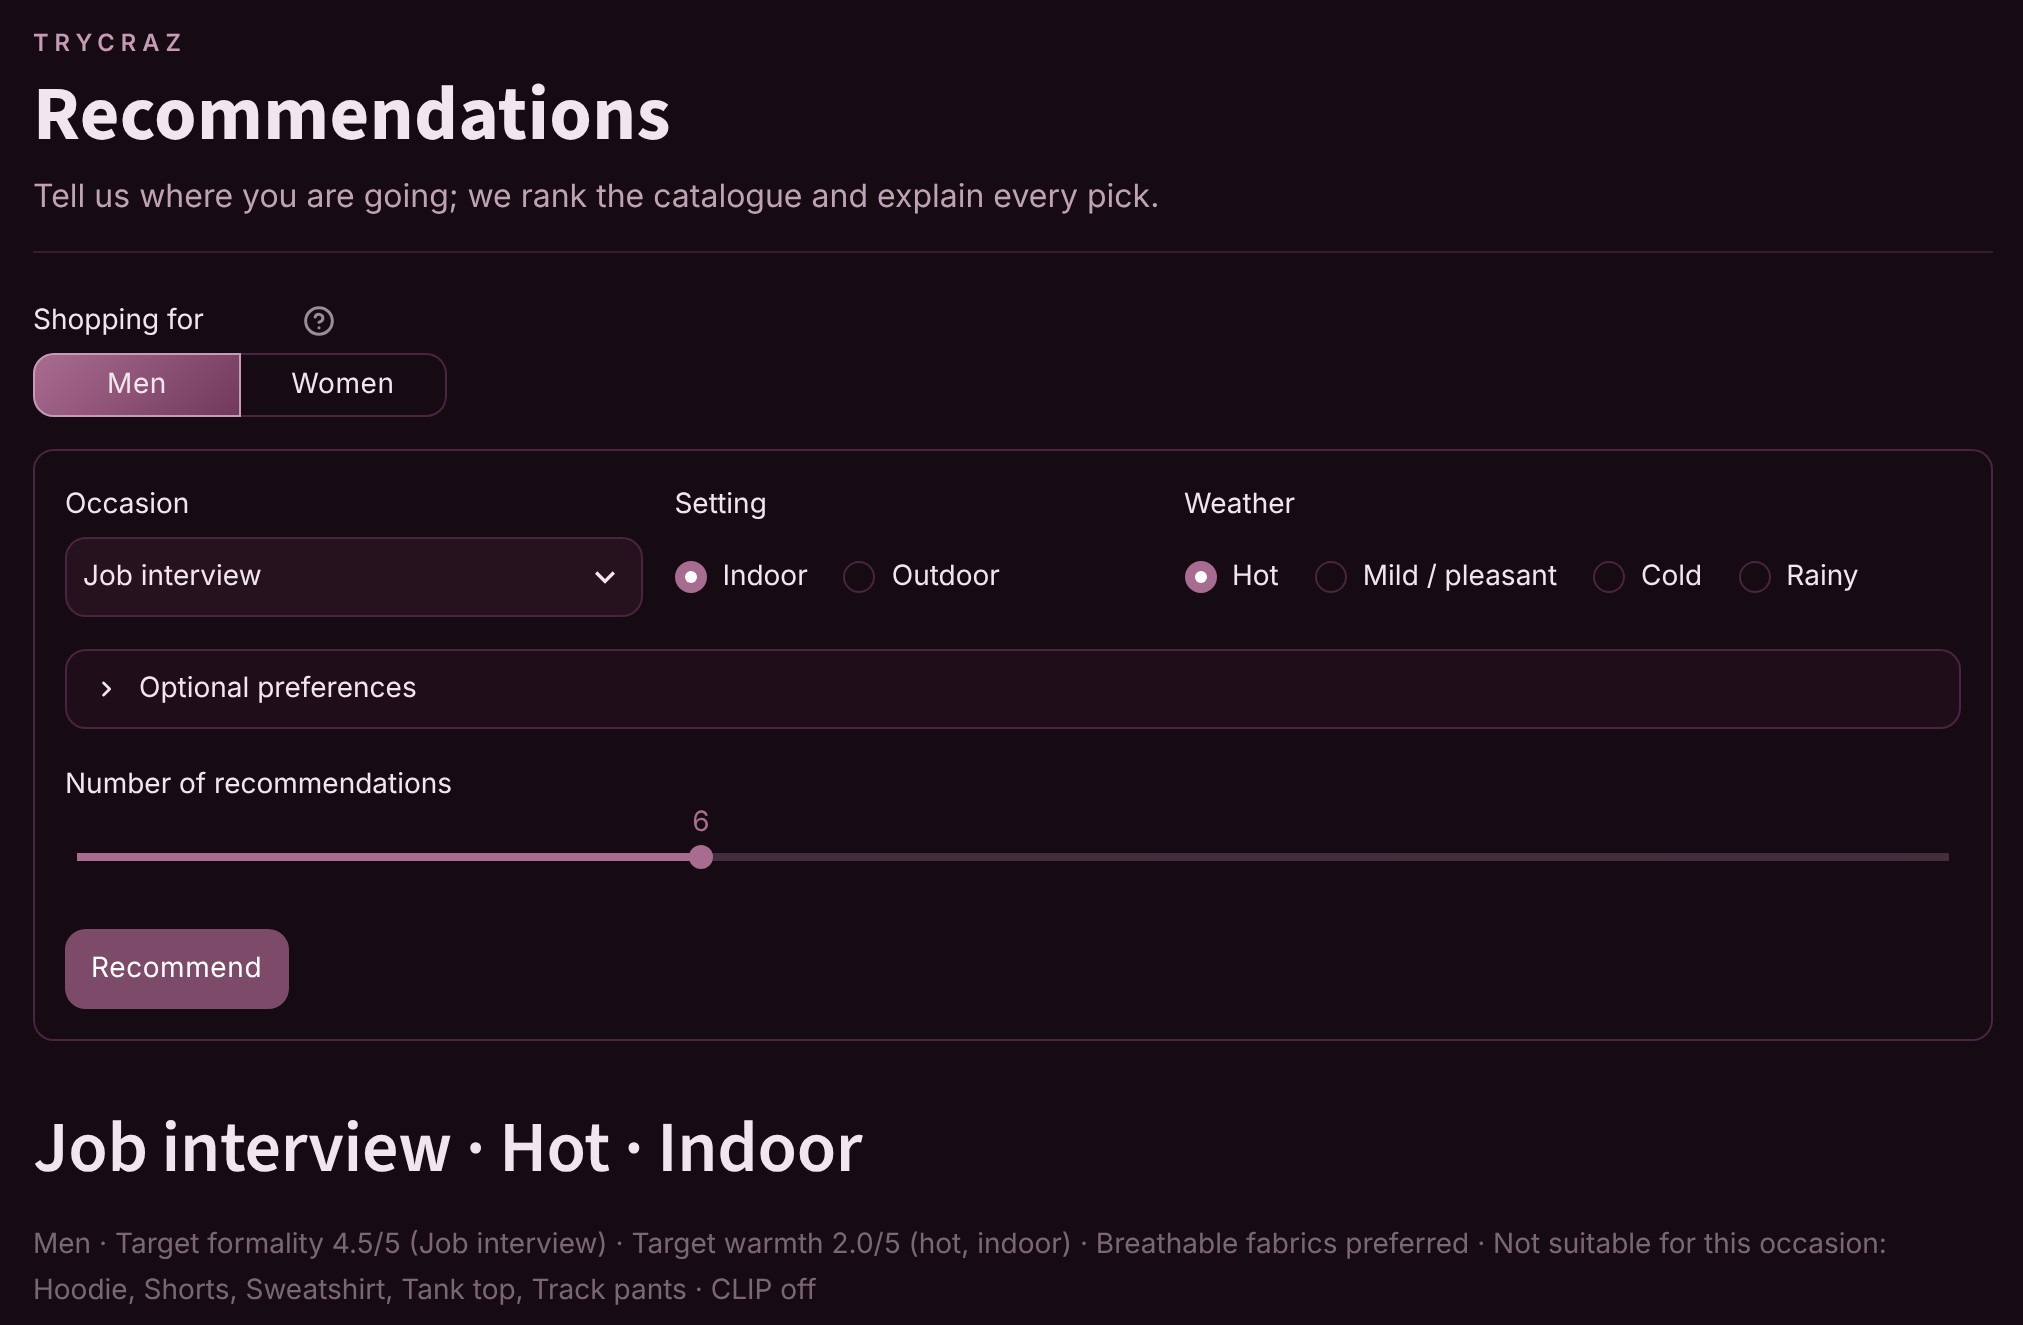
\includegraphics[width=0.493\textwidth]{figs/app_form.jpg}\hfill
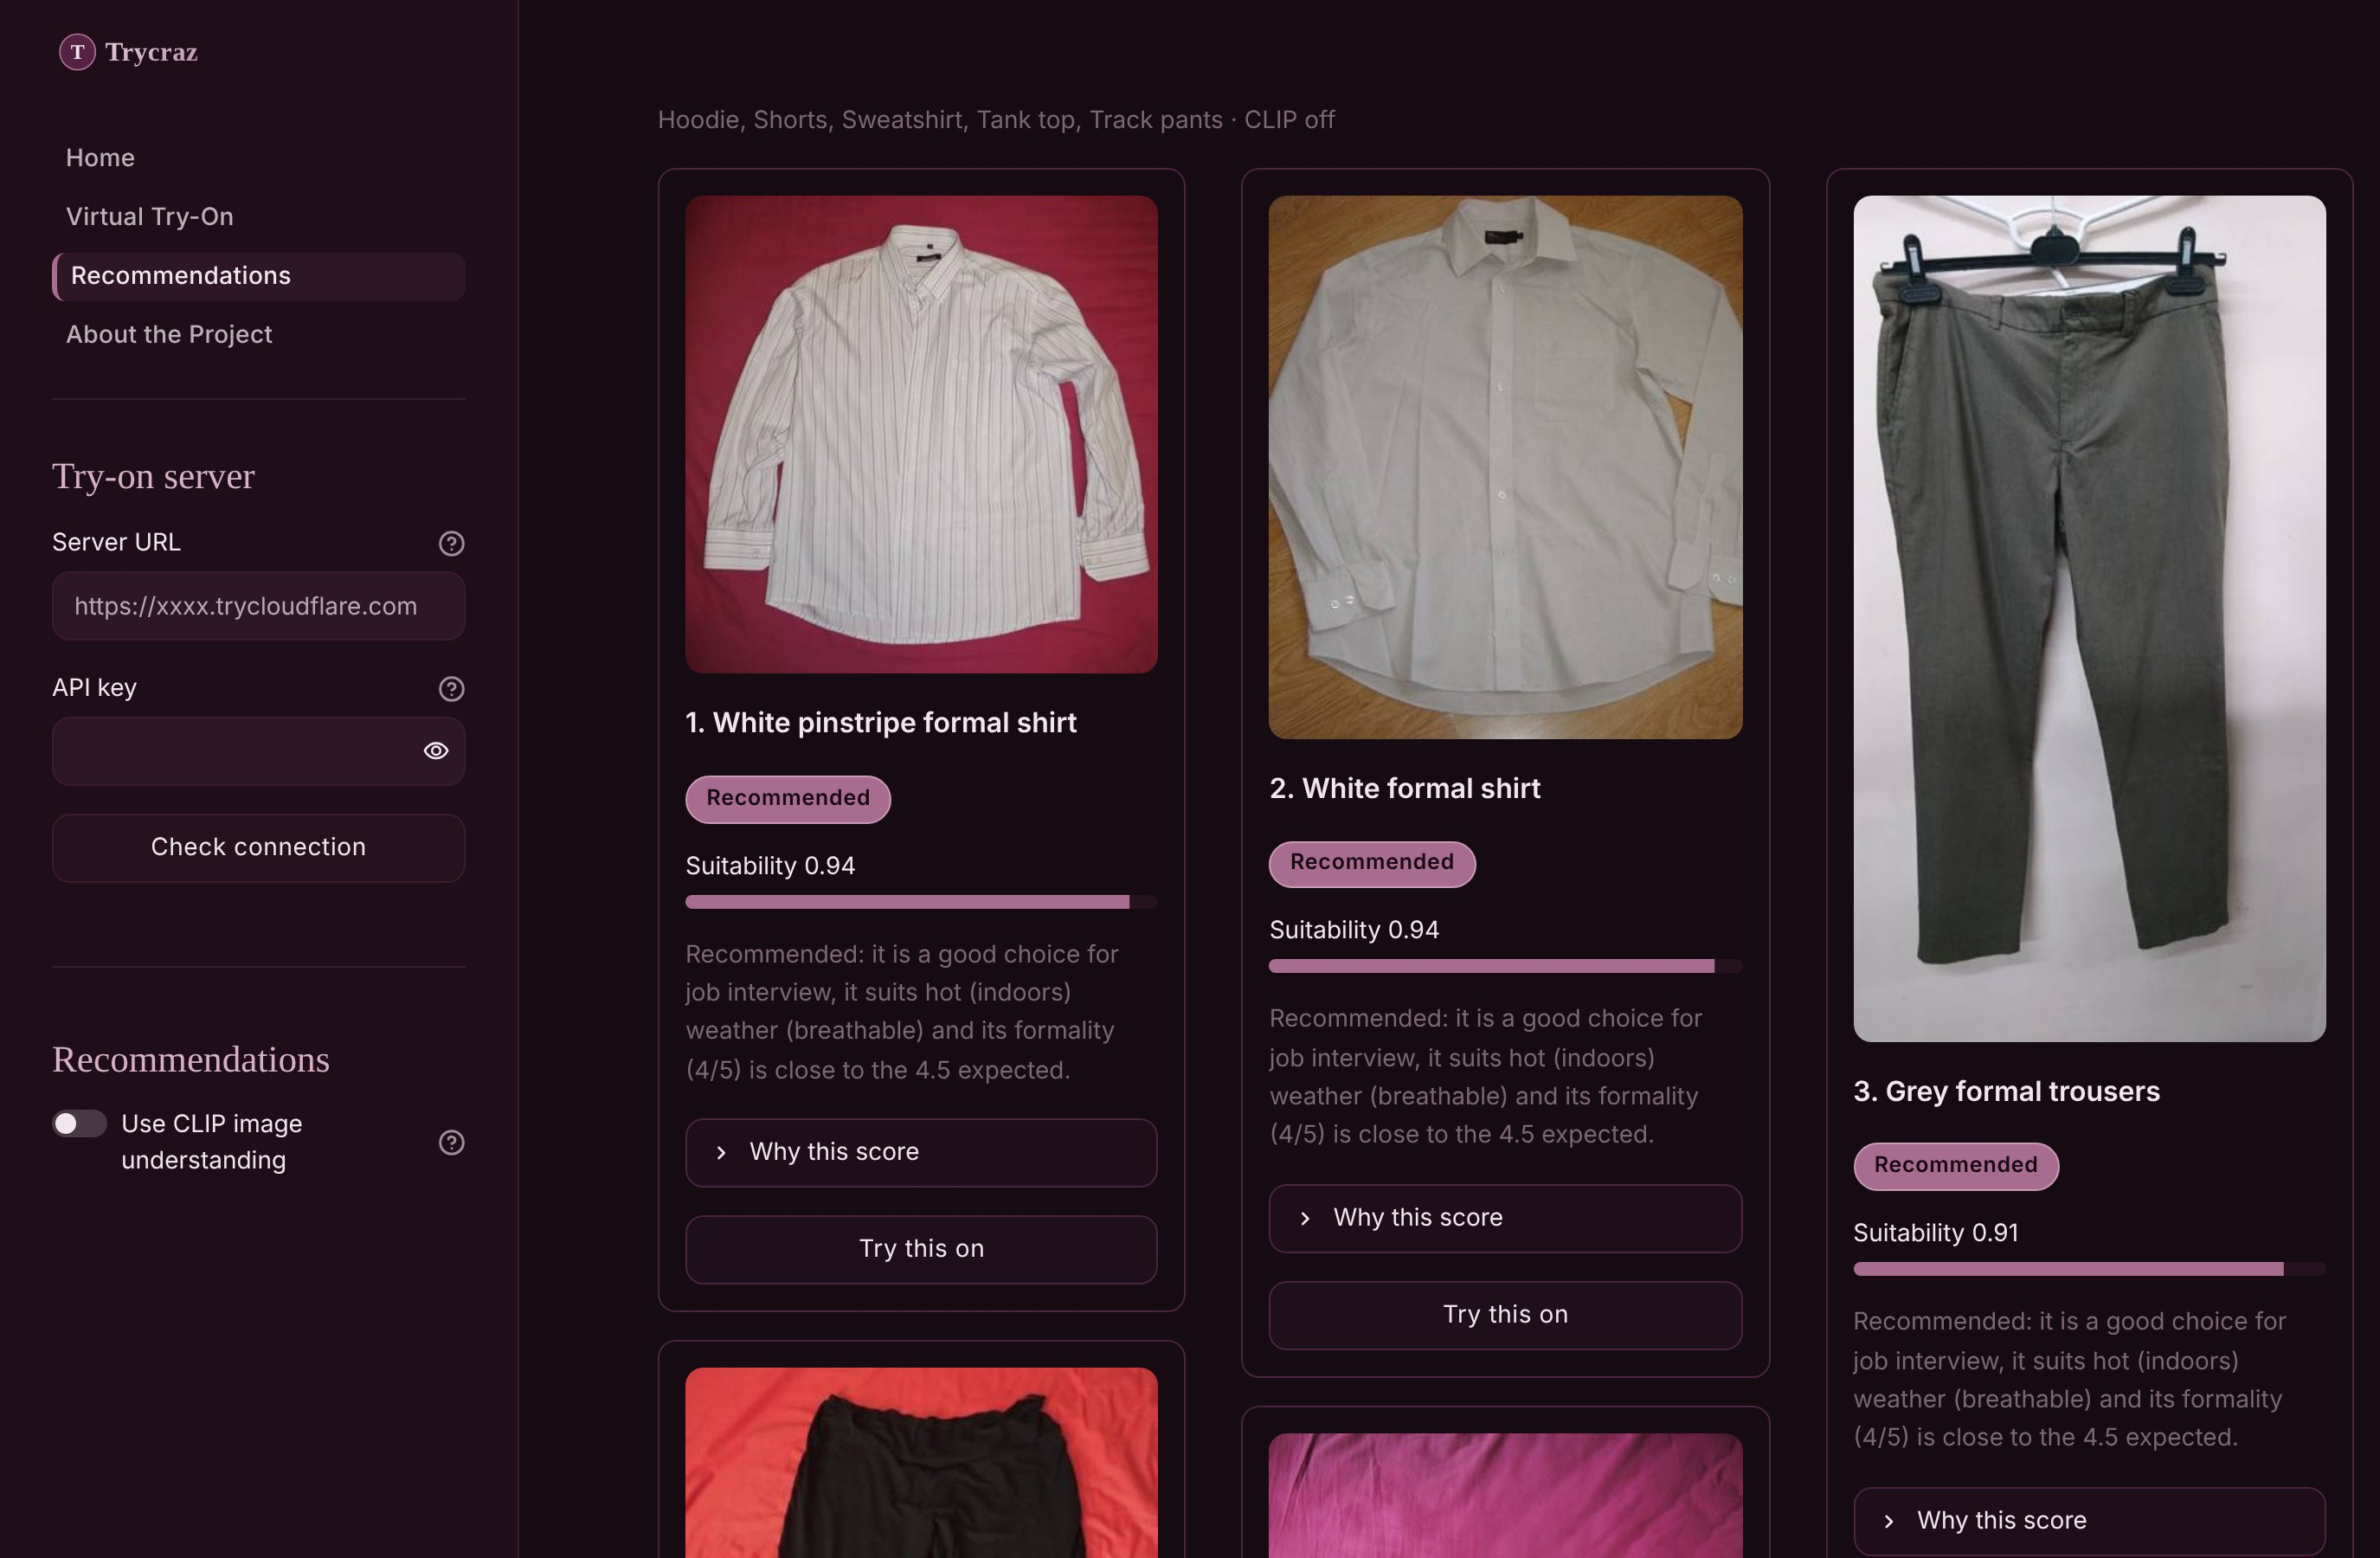
\includegraphics[width=0.493\textwidth]{figs/app_cards.jpg}
\caption{The Recommendations page. Left: the user picks Men or Women, then the occasion, setting and
weather (here a job interview, indoors, hot). Right: ranked cards with verdict, score, explanation,
a breakdown of the six factors and a button that opens the garment in the try-on page.}
\label{fig:app}
\end{figure}


\section{Experiments and Results}
\label{sec:exp}

\subsection{Setup}

Try-on ran on a free Colab T4 with CatVTON at a pinned commit, \texttt{mix-48k-1024} weights, fp16,
768$\times$1024, 30 DDIM steps, guidance 2.5, seed 42 and repaint on. The client was a Windows laptop
(Intel i5-12450H, 7.6\,GB RAM) connected over the tunnel. Try-on quality was judged by eye, since we
have no ground truth image for a new person--garment pair.

\subsection{Speed and Memory}

Table~\ref{tab:perf} summarises ten runs. The diffusion loop is almost all of the server time; masking
takes about a second. The round trip seen by the user varies more because it includes uploading,
the tunnel and waiting in the queue behind another job.

\begin{table}[t]
\caption{Try-on performance on a T4 (10 runs, 30 steps)}
\label{tab:perf}
\centering
\begin{tabular}{@{}lr@{}}
\toprule
Measure & Value\\
\midrule
Diffusion, 30 steps & 61.5--62.4\,s ($\approx$2.1\,s/step)\\
Mask (DensePose + 2$\times$SCHP) & 0.94--1.36\,s\\
Peak GPU memory & 4.89\,GB of 15\,GB\\
Round trip from the laptop & 69--133\,s\\
Model load, once per session & 86\,s\\
\bottomrule
\end{tabular}
\end{table}

\subsection{Try-On Quality}

Our first six real runs with home-style garment photos (R2--R7 in Table~\ref{tab:runs}) gave two
successes, two partial results and two failures. After the two fixes described next, we ran six
validation try-ons with full-body photos and background-removed catalogue garments, and all six
succeeded (Fig.~\ref{fig:tryon}). The blazer keeps its lapels and button, the elephant print on the
T-shirt survives, the jeans keep their fading, and in every case the face, hands, shoes and background
are unchanged. The remaining flaws are small: the blazer comes out slightly lighter than the original,
the white shirt looks a little sheer, and the T-shirt's sleeves end higher than the sweater's did, so
the model has to invent the forearms.

\begin{table}[t]
\caption{Real try-on runs, judged by eye}
\label{tab:runs}
\centering
\setlength{\tabcolsep}{3pt}
\begin{tabular}{@{}llll@{}}
\toprule
Run & Garment (photo background) & Type & Result\\
\midrule
R2 & navy blazer (door, pink wall) & upper & failure\\
R3 & white formal shirt (wooden floor) & upper & failure\\
R4 & white wrap blouse (white wall) & upper & success\\
R5 & black trousers (red bedsheet) & lower & partial\\
R6 & light blue jeans (beige sheet) & lower & success\\
R7 & tropical print dress (wooden floor) & overall & partial\\
\midrule
V1--V6 & six catalogue garments (bg.\ removed) & all & 6/6 success\\
\bottomrule
\end{tabular}
\end{table}

\begin{figure}[t]
\centering
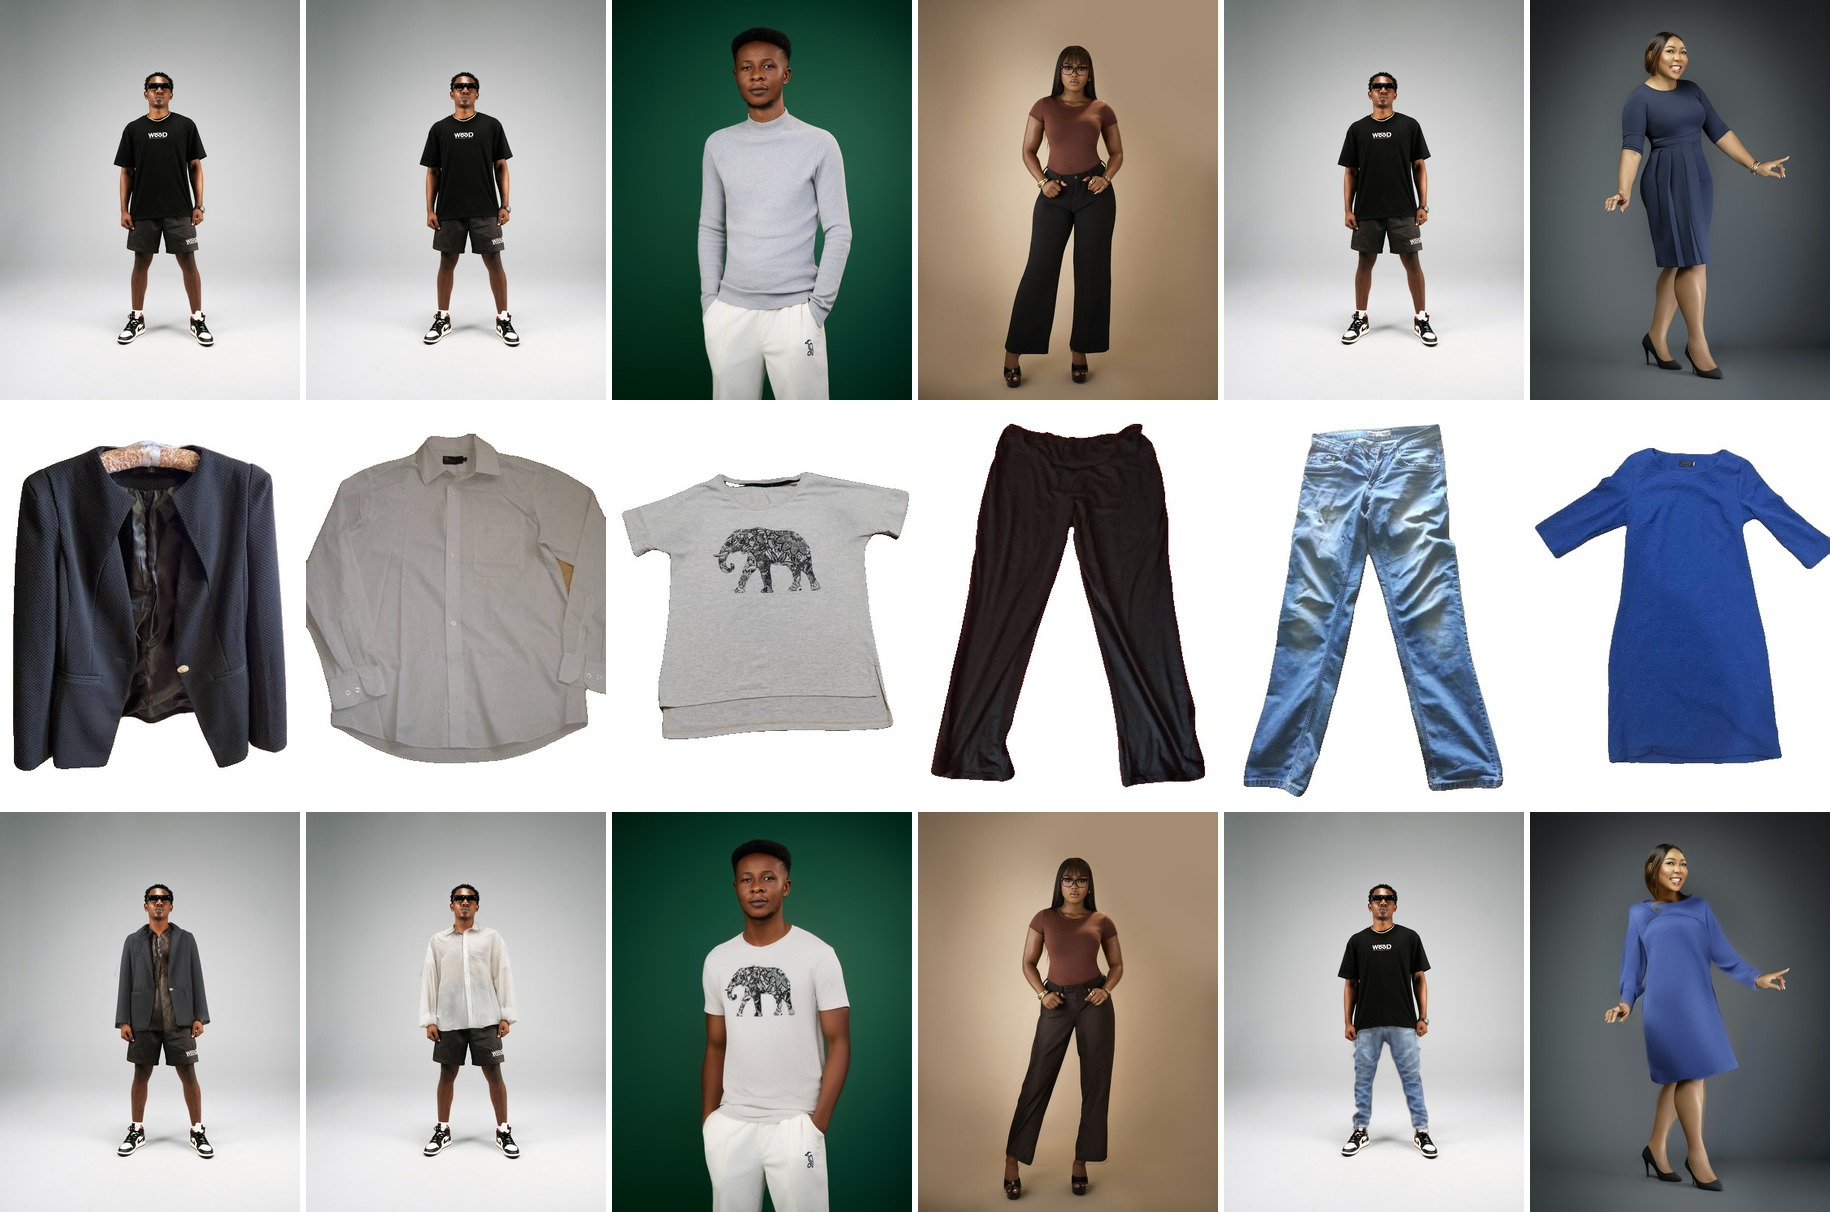
\includegraphics[width=\textwidth]{figs/tryon_grid.jpg}
\caption{Validation try-ons V1--V6 generated by CatVTON on a T4 through our pipeline. Rows: input
person, garment after our background removal, result. Columns: navy blazer, white formal shirt, printed
T-shirt (all upper body), black formal trousers, light blue jeans (lower body) and a royal blue sheath
dress (full outfit).}
\label{fig:tryon}
\end{figure}

\subsection{Failure Diagnosis}
\label{sec:diag}

Runs R2 and R3 put a blazer and a formal shirt on the same man, and both came out as a grey, knitted
looking top with a pale halo around the shoulders (Fig.~\ref{fig:diag}a--c). We tested one hypothesis
at a time, keeping the seed and settings fixed (Table~\ref{tab:diag}).

\begin{table}[t]
\caption{Diagnosing R2/R3: hypothesis, test, evidence}
\label{tab:diag}
\centering
\setlength{\tabcolsep}{3pt}
\begin{tabular}{@{}>{\raggedright\arraybackslash}p{3.3cm}>{\raggedright\arraybackslash}p{5.1cm}>{\raggedright\arraybackslash}p{4.9cm}@{}}
\toprule
Hypothesis & Test & Evidence\\
\midrule
Cluttered garment background & remove it with \unet, rerun & still grey with a halo (d): rejected\\
The garment is the problem & same blazer on two other people & correct blazer both times (e, f): rejected\\
The person photo is the problem & a T-shirt that worked before, on this man & top half fine, bottom half grey (g): confirmed\\
Why this photo? & MediaPipe hip height on the 3:4 crop & failing: 0.89, 0.91; working: 0.43--0.50\\
\bottomrule
\end{tabular}
\end{table}

\begin{figure}[t]
\centering
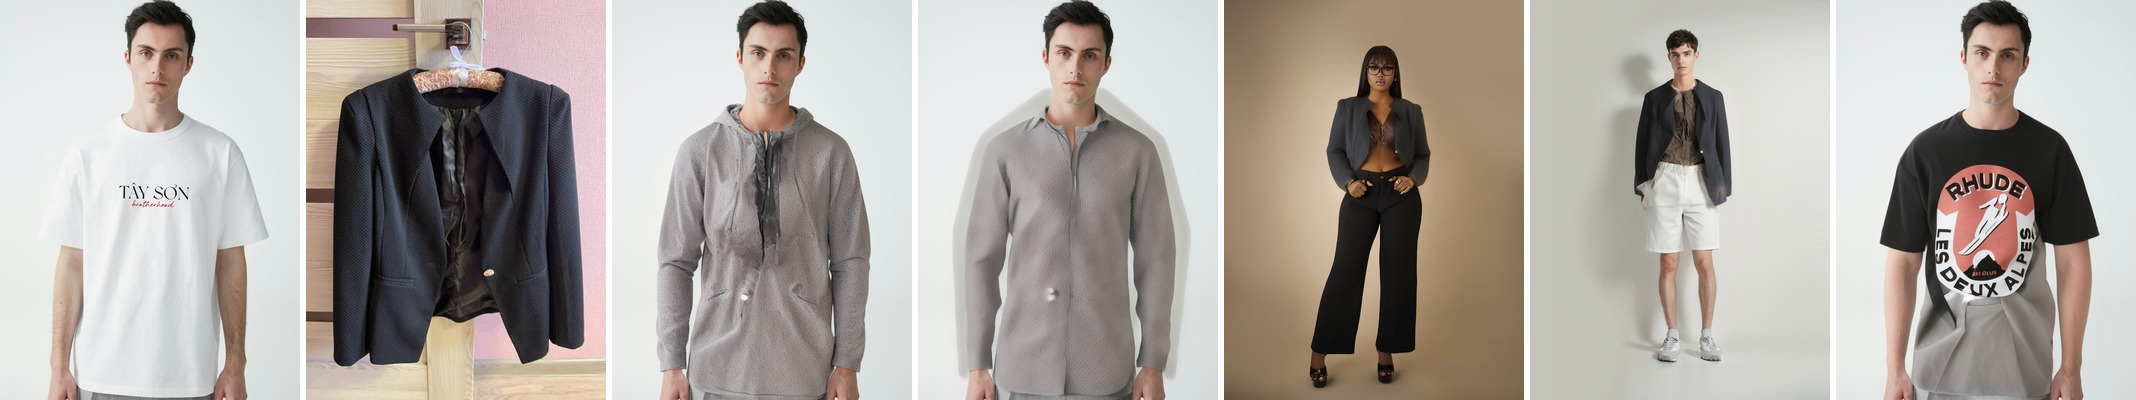
\includegraphics[width=\textwidth]{figs/diag_hips.jpg}\\[1pt]
\tl{(a) input}\tl{(b) garment}\tl{(c) R2 result}\tl{(d) bg.\ removed}\tl{(e) other person}\tl{(f) other person}\tlast{(g) known-good tee}\\[4pt]
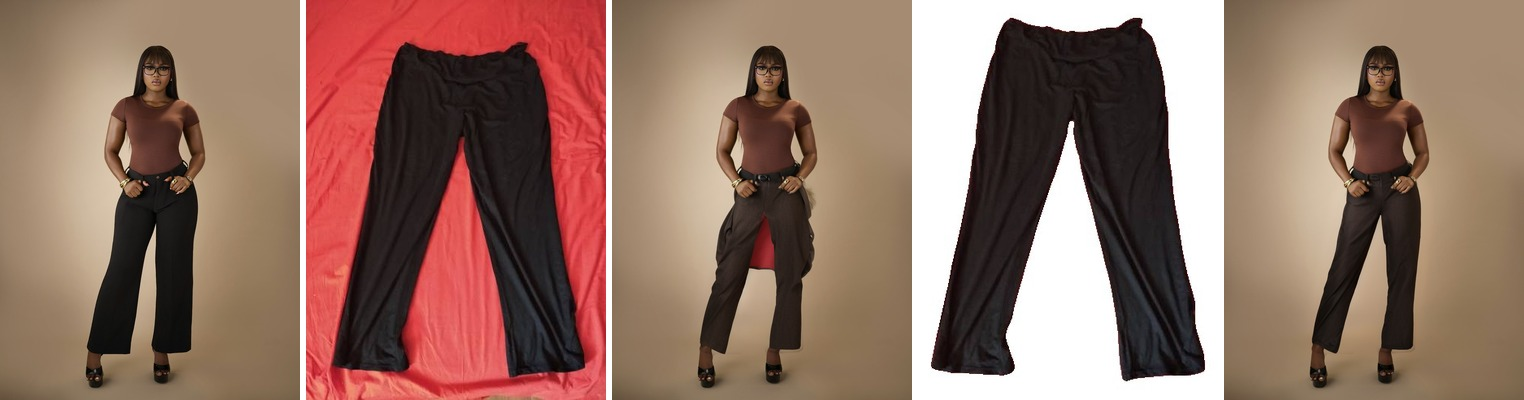
\includegraphics[width=0.714\textwidth]{figs/diag_bleed.jpg}\\[1pt]
\tl{(h) input}\tl{(i) on a red sheet}\tl{(j) R5 result}\tl{(k) bg.\ removed}\tlast{(l) V3 result}
\caption{Failure analysis. Top: the man's photo ends at the hips. The blazer fails on him with or without
its background (c, d), works on two other people (e, f), and even a T-shirt that worked before fails on him
in the lower half (g). Bottom: the red bedsheet behind the trousers leaks into the result (j); after
background removal the trousers come out clean (l).}
\label{fig:diag}
\end{figure}

The photo of this man ends at the hips, so the region to repaint touches the bottom edge of the image.
For a long garment there is no body below the hem to anchor it, and the model fills the missing part
with grey. We turned this into the \texttt{cut\_off\_at\_hips} rule in Table~\ref{tab:rules} and moved
the photo out of our samples into a folder of failure examples. A second problem showed up in R5: the
black trousers had been photographed on a red bedsheet, and red patches appeared inside the generated
trousers (Fig.~\ref{fig:diag}j). Background removal fixed this (l), which is why we kept it even though
it was not the cause of R2.

\subsection{Recommendation Quality}

We wrote twelve test scenarios, each a context plus graded relevance labels for the catalogue (2 = good
choice, 1 = acceptable, unlisted = unsuitable). The labels were written from the garment photos and names
\emph{before} the recommender was run on this catalogue. With $k=5$, Precision@5 is the share of the top
five with relevance at least 1, and
\begin{equation}
\text{nDCG@}k=\frac{1}{\text{IDCG@}k}\sum_{i=1}^{k}\frac{2^{r_i}-1}{\log_2(i+1)},
\end{equation}
where $r_i$ is the relevance of the item at rank $i$ and IDCG is the same sum for the ideal order, so
nDCG also rewards putting the best items first.

\begin{table}[t]
\caption{Recommender ablation (12 scenarios, $k=5$, real CLIP)}
\label{tab:rec}
\centering
\begin{tabular}{@{}lcc@{}}
\toprule
Configuration & Mean P@5 & Mean nDCG@5\\
\midrule
Attributes only (no CLIP) & 0.767 & 0.751\\
CLIP only & 0.667 & 0.691\\
\textbf{Hybrid (default weights)} & \textbf{0.833} & \textbf{0.830}\\
\bottomrule
\end{tabular}
\end{table}

\begin{figure}[t]
\centering
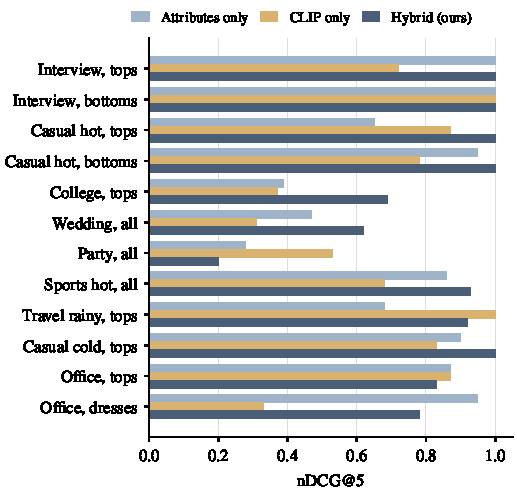
\includegraphics[width=0.62\linewidth]{figs/ndcg_per_scenario.pdf}
\caption{nDCG@5 per scenario for the three configurations. The hybrid is best or tied in 8 of 12
scenarios. In Party, Travel, Office tops and Office dresses one signal alone does better.}
\label{fig:ndcg}
\end{figure}

Table~\ref{tab:rec} shows the ablation and Fig.~\ref{fig:ndcg} the per-scenario results. The hybrid
beats both of its parts on average. The two signals fail in different places. The attribute rules are
weak on College tops (nDCG 0.39), where a rain jacket and a camisole reach the top five because their
occasion tags are broad, and on Party (0.28). CLIP alone is weak on Wedding (0.31) and Office dresses
(0.33), where it cannot tell a smart dress from a casual one in a flat photo, but it is perfect on Travel
in the rain, where a rain jacket simply looks like a rain jacket. Combined, College rises to 0.69 and
Wedding to 0.62.

To check that the ranking really depends on the context, we computed Kendall's $\tau$ between the
rankings of every pair of scenarios that share at least five garments (45 pairs). The mean is 0.01 for
the hybrid (0.07 for attributes only), where $\tau=1$ would mean the same order whatever the occasion.
Party is the weakest scenario for both the hybrid (0.20) and the rules (0.28). ``Party wear'' covers
very different garments, and our catalogue has few of them. In four scenarios one signal alone ranks
better than the mix, which suggests the weights are reasonable but not optimal; we chose not to tune
them on these labels (Section~\ref{sec:opt}).

\subsection{Automatic Garment Annotation}

For uploaded garments the attributes come from the photo. We compared the automatic estimates with our
manual labels on all 52 catalogue garments (Table~\ref{tab:auto}). Background removal mainly helps colour,
because bedsheet and floor pixels no longer enter the colour clusters. Garment type is harder than it
looks: several classes are genuinely close (polo and T-shirt, jacket and blazer, sweater and sweatshirt).

\begin{table}[t]
\caption{Automatic vs.\ manual annotation (52 garments)}
\label{tab:auto}
\centering
\setlength{\tabcolsep}{4pt}
\begin{tabular}{@{}lcc@{}}
\toprule
Measure & Before bg.\ removal & After\\
\midrule
Type, CLIP top-1 (26 classes) & 32/52 (62\%) & 33/52 (63\%)\\
Main colour, k-means name & 26/52 (50\%) & 30/52 (58\%)\\
\bottomrule
\end{tabular}
\end{table}

\subsection{Software Testing}
\label{sec:tests}

The project has 166 automated tests, and all pass on the laptop and on Linux. They cover input
validation with broken and unusual files, the crop arithmetic against CatVTON's own function, the
server's job life-cycle and every error code, the laptop client against a real local server, the pose
rules on synthetic landmarks, the recommender's behaviour in typical scenarios, the metrics against
hand-computed values and the four app pages. One test generates explanations for all 9 occasions and 4
weather types and checks that no stated reason contains negative wording, which guards the bug mentioned
in Section~\ref{sec:rec}. CatVTON's own code was also run end to end with randomly initialised weights
on the CPU, which confirmed that it works on Python 3.12 before we spent any GPU time. Against the real
server, a wrong API key, an unreachable URL and a queued second request all produced the intended
messages.

\subsection{Discussion and Limitations}
\label{sec:disc}

\emph{What worked.} The split between a laptop and a free cloud GPU made a 899\,M-parameter model usable
without any lab hardware, at the cost of about a minute per image and a session that has to be
restarted every few hours. The most useful part of the try-on pipeline turned out to be the checks
\emph{before} generation. CatVTON itself was reliable once its inputs looked like its training data:
a front-facing person with body visible below the garment, and a garment on a plain background. Both
of our failures were input problems, and both are now caught or fixed automatically.

\emph{Why the hybrid helps.} Rules and CLIP make different mistakes. The rules know conventions that
cannot be seen in a photo, such as shorts not being worn to an interview, but they rely on our tags.
CLIP sees the actual garment but is easily fooled by photo style. A weighted sum lets each correct the
other, and because the explanation comes from the same factor values, the user can see which signal
drove each decision.

\emph{Limitations.} We should be clear about what our numbers do and do not show.
\begin{itemize}
\item Try-on quality was judged by eye on twelve runs. We have not yet computed paired metrics such as
SSIM, LPIPS or KID on the VITON-HD test set; for reference, the CatVTON authors report SSIM 0.870 and
LPIPS 0.057 there~\cite{catvton}.
\item The recommender labels come from a single annotator who also wrote the knowledge base and the
catalogue tags, so the scores are probably optimistic. Twelve scenarios and 52 garments are small.
\item The catalogue images are only 400\,px wide, which limits fine detail, and there is no
traditional Indian wear such as kurtas or sarees. Draped garments like sarees are outside what this
model supports.
\item The dress-code rules are hand-written and culturally specific. The app presents its output as
suggestions, not rules.
\item A free cloud GPU can disconnect, and each new session spends a few minutes downloading and loading the model.
\end{itemize}

\emph{Licences.} CatVTON is released under CC BY-NC-SA 4.0, so Trycraz is for academic,
non-commercial use. All photos we used are CC0 or under the Unsplash licence, and credits are listed in
the app.

\emph{Future work.} The next steps follow from the limitations: run the paired VITON-HD metrics on a
T4; have a second person label the scenarios independently and report the agreement; photograph our
own clothes on a plain background to replace the low-resolution catalogue images; and add a short
user study in which people rate realism and suitability.


\section{Conclusions}
\label{sec:concl}

Trycraz shows that realistic virtual try-on and context-aware recommendation can be combined in one
working system built on free hardware. A pretrained CatVTON model generates the images on a cloud T4 in
about 62\,s with under 5\,GB of GPU memory, while our own pipeline decides whether a photo is good
enough to send, cleans the garment photo and handles the long-running job over an unreliable tunnel.
Diagnosing our failures step by step showed that input framing, not the garment or the model, caused
them, and after adding a framing rule and background removal all six validation try-ons succeeded. The
hybrid recommender, which adds CLIP's view of the photo to hand-written dress-code rules, reached a mean
P@5 of 0.833 and nDCG@5 of 0.830, better than either part alone, and explains every score from the same
numbers that produced it. The main gaps are evaluation gaps, namely paired image metrics and independent
labels, and they are the first things we would add.

\emph{Code availability.} The full source code, setup guide, test suite and evaluation scripts are
public at \url{https://github.com/CrazAzartto/trycraz-virtual-tryon}.


{\small
\begin{thebibliography}{9}

\bibitem{catvton}
Z.~Chong \emph{et al.}, ``CatVTON: Concatenation is all you need for virtual try-on with diffusion
models,'' in \emph{Proc. ICLR}, 2025.

\bibitem{ldm}
R.~Rombach, A.~Blattmann, D.~Lorenz, P.~Esser, and B.~Ommer, ``High-resolution image synthesis with
latent diffusion models,'' in \emph{Proc. IEEE CVPR}, 2022, pp. 10684--10695.

\bibitem{vitonhd}
S.~Choi, S.~Park, M.~Lee, and J.~Choo, ``VITON-HD: High-resolution virtual try-on via
misalignment-aware normalization,'' in \emph{Proc. IEEE CVPR}, 2021, pp. 14131--14140.

\bibitem{idmvton}
Y.~Choi, S.~Kwak, K.~Lee, H.~Choi, and J.~Shin, ``Improving diffusion models for authentic virtual
try-on in the wild,'' in \emph{Proc. ECCV}, 2024.

\bibitem{densepose}
R.~A.~G{\"u}ler, N.~Neverova, and I.~Kokkinos, ``DensePose: Dense human pose estimation in the wild,''
in \emph{Proc. IEEE CVPR}, 2018, pp. 7297--7306.

\bibitem{schp}
P.~Li, Y.~Xu, Y.~Wei, and Y.~Yang, ``Self-correction for human parsing,'' \emph{IEEE Trans. Pattern
Anal. Mach. Intell.}, vol.~44, no.~6, pp. 3260--3271, 2022.

\bibitem{blazepose}
V.~Bazarevsky, I.~Grishchenko, K.~Raveendran, T.~Zhu, F.~Zhang, and M.~Grundmann, ``BlazePose:
On-device real-time body pose tracking,'' arXiv:2006.10204, 2020.

\bibitem{u2net}
X.~Qin, Z.~Zhang, C.~Huang, M.~Dehghan, O.~R.~Zaiane, and M.~Jagersand, ``U$^2$-Net: Going deeper with
nested U-structure for salient object detection,'' \emph{Pattern Recognit.}, vol.~106, p.~107404, 2020.

\bibitem{clip}
A.~Radford \emph{et al.}, ``Learning transferable visual models from natural language supervision,''
in \emph{Proc. ICML}, 2021, pp. 8748--8763.

\end{thebibliography}
}
\end{document}
